\section{Objetivo de evaluación}
El objetivo de esta sección es definir una metodología que permita evaluar la calidad de un conjunto de historias de usuario generadas automáticamente por un modelo de lenguaje (LLM) a partir de un documento de requisitos de producto (PDR).

Con esta evaluación se busca determinar si las historias de usuario generadas tienen la calidad necesaria y suficiente como para ser utilizadas en procesos de desarrollo de software y si representan adecuadamente el dominio funcional definido en el documento de requisitos desde el que fueron generadas. Se busca determinar adicionalmente en qué medida el conjunto de historias generado se aproxima a una solución construida manualmente por analistas humanos para el mismo dominio, y también detectar posibles inconsistencias o contenido incorrecto introducido durante la generación automática.

El estudio en conjunto de estas dimensiones nos permite determinar un veredicto para las historias de usuario generadas, considerando tanto la utilidad práctica en el desarrollo de software, coherencia interna de cada historia, su fidelidad con las demás historias del conjunto y su correspondencia con el dominio del documento de requisitos.

\section{Aspectos de calidad evaluados}

El análisis de calidad de las historias de usuario se basa en el Quality User Story Framework (QUSF), el cual define tres dimensiones fundamentales de calidad: sintáctica, semántica y pragmática. Este framework permite evaluar las propiedades internas de las historias de usuario sin considerar aún su correspondencia con la fuente de origen.
Sin embargo, como uno de los objetivos de este trabajo es evaluar también la fidelidad de las historias generadas respecto al documento de requisitos del producto (PDR), se incorporan además aspectos relacionados con la relación entre las historias generadas y el documento de requisitos, como la correctitud de la solución respecto a la fuente de información, cobertura del dominio funcional y trazabilidad entre las historias generadas y los requisitos del documento. Esto nos permite analizar cómo se corresponden las historias generadas y el documento de requisitos desde dos perspectivas complementarias. Por un lado con la correctitud evaluamos si las historias generadas se corresponden correctamente a las funcionalidades definidas para el dominio, y para la cobertura estudiamos si las funcionalidades del dominio se encuentran presentes en el conjunto de historias generadas. Para esto es necesario contar con un ground truth que contemple coherentemente el dominio, por lo que se generan tanto historias de usuario esperadas como funcionalidades extraídas del PDR, con el objetivo de medir qué porcentaje de este dominio es cubierto por las historias generadas.
Adicionalmente fue incorporado a la evaluación el criterio INVEST como un análisis complementario. Si bien QUSF permite analizar la calidad estructural y conceptual de las historias, INVEST introduce criterios relevantes para su uso práctico dentro de procesos ágiles, tales como independencia, negociabilidad o estimabilidad, que no se encuentran completamente contemplados en el QUSF. 
\newline

Se definen entonces las siguientes dimensiones para la evaluación.
\paragraph{Calidad de las historias de usuario (QUSF)}
Este aspecto evalúa las propiedades internas de las historias de usuario, tanto a nivel individual como a nivel del conjunto. Siguiendo las dimensiones propuestas por QUSF, se consideran tres tipos de calidad. La calidad sintáctica analiza la estructura textual de las historias sin considerar su significado, incluyendo aspectos como la gramática, la redacción y el cumplimiento de la estructura esperada. La calidad semántica evalúa el significado del contenido, verificando que las historias sean claras, consistentes y correctamente relacionadas dentro del dominio del problema. Finalmente, la calidad pragmática analiza cómo las historias pueden ser interpretadas por los desarrolladores y si resultan adecuadas para su uso dentro de procesos de desarrollo.
\paragraph{Usabilidad en contexto ágil (INVEST)}
Este aspecto evalúa si las historias de usuario cumplen los criterios definidos por el modelo INVEST: Independent, Negotiable, Valuable, Estimable, Small y Testable. Estos criterios permiten analizar si las historias generadas pueden ser utilizadas adecuadamente dentro de metodologías ágiles de desarrollo.
\paragraph{Correctitud respecto al PDR}
Este criterio evalúa la fidelidad de las historias generadas con respecto al documento de requisitos del producto. En particular, se analiza si las historias generadas describen funcionalidades que efectivamente existen dentro del PDR. Este análisis permite identificar casos en los que el modelo genera historias que introducen elementos o funcionalidades no presentes en el documento original, fenómeno conocido como alucinación.
\paragraph{Cobertura del dominio}
Este aspecto evalúa en qué medida el conjunto de historias generadas cubre las funcionalidades esperadas del sistema definidas en el documento de requisitos. El objetivo de este análisis es determinar si existen funcionalidades del dominio que no fueron representadas por ninguna historia generada, lo que permite identificar posibles omisiones en la generación automática.
\paragraph{Trazabilidad}
Finalmente, se evalúa la correspondencia entre las historias generadas y los requerimientos del PDR, verificando si cada historia puede vincularse con la sección del documento a partir de la cual fue derivada.

\section{Cómo se evalúa cada aspecto}
%Cómo evaluamos cada aspecto, las tablas de SI o No, si se sus 1 al 5 Sbert, implementación
Como se comentó en el Capítulo \ref{cap:central} Sección \ref{central-enfoque}, en el estudio de \cite{yu2026evaluating_genai_quality_multicase} se identifican tres maneras de evaluar soluciones creadas con inteligencia artificial, de manera automática, de manera manual por analistas o expertos en el área y de manera asistida.

Para las evaluaciones manuales existen estrategias como Reviewer scorecard utilizando una escala como Likert.

El criterio INVEST es analizado de manera manual por nosotros, como analistas expertos. Seguiremos la estrategia Reviewer scorecard, para cada aspecto de INVEST se asigna un puntaje de la escala Likert (1 al 5) donde (1 = muy deficiente, 3 = aceptable, 5 = excelente). De esta manera se obtiene para cada aspecto de INVEST un puntaje evaluado para cada historia.
Aplicamos también la evaluación del criterio SMALL, agregando la clasificación de Épica a la evaluación, para contabilizar las historias que abarcan más de una funcionalidad y por lo tanto requieren refinamiento.

Los criterios presentados por QUSF, son evaluados manual y automáticamente. Criterios de carácter sintáctico son evaluados utilizando la implementación parcial del esquema de evaluación propuesto, presentado por los mismos autores: AQUSA \cite{aqusa}.
Esta implementación cubre los criterios sintácticos de atomicidad, minimal y buen formato. Además de cubrir aspectos pragmáticos de unicidad (detección de duplicado exacto), uniforme (mismo formato en el conjunto de historias).
Estos criterios son entonces analizados de manera automática corriendo la aplicación que toma como entrada la lista de historias de usuario, sin incluir criterios de aceptación y devuelve la lista de defectos por historia.
El resto de criterios presentados en el esquema de evaluación QUSF son detectados de manera manual. Por simplicidad y dado que cada criterio tiene una descripción clara, descritos en la Tabla \ref{table:qusf}, se marca SI o No a su cumplimiento, por historia para aquellos que evalúan a nivel individual y para el conjunto.

\begin{longtable}{|l|p{6cm}|p{2cm}|}
\caption{Criterios de Quality User Story framework (QUSF)}
\label{table:qusf} \\
\hline
\textbf{Criteria} & \textbf{Descripción} & \textbf{Individual o Conjunto} \\
\hline

\multicolumn{3}{|l|}{Syntactic} \\ \hline
Well-formed & Una historia de usuario incluye al menos un rol y un medio. & Individual \\ \hline
Atomic & Una historia expresa un requisito para exactamente una funcionalidad. & Individual \\ \hline
Minimal & Una historia contiene únicamente rol, medio y fin. & Individual \\ \hline

\multicolumn{3}{|l|}{Semantic} \\ \hline
Conceptually sound & El medio expresa una funcionalidad y el fin expresa una justificación. & Individual \\ \hline
Problem-oriented & La historia especifica solo el problema, no la solución. & Individual \\ \hline
Unambiguous & Evita términos o abstracciones que permitan múltiples interpretaciones. & Individual \\ \hline
Conflict-free & No es inconsistente con otras historias de usuario. & Conjunto \\ \hline

\multicolumn{3}{|l|}{Pragmatic} \\ \hline
Full sentence & Es una oración completa y bien formada. & Individual \\ \hline
Estimable & No representa un requisito demasiado amplio difícil de planificar. & Individual \\ \hline
Unique & Cada historia es única; se evitan duplicados. & Conjunto \\ \hline
Uniform & Todas las historias emplean la misma plantilla. & Conjunto \\ \hline
Independent & La historia es autocontenida y no depende de otras historias. & Conjunto \\ \hline
Complete & El conjunto de historias permite una aplicación completa sin pasos faltantes. & Conjunto \\ \hline
\end{longtable}

La cobertura del documento de requisitos será analizada de manera automática, utilizando un algoritmo de similitud semántica, Sentence BERT \cite{reimers-2019-sentence-bert}. Se mide la similitud semántica historia por historia con respecto a una solución construida por nosotros, como analistas expertos, para el dominio presentado. Se tiene entonces, el conjunto de historias generadas y el conjunto de historias esperadas, donde las historias generadas por la herramienta deben corresponder a las historias esperadas en la solución completa.
Sentence BERT calcula la similitud entre oraciones y devuelve un valor, lo que permite definir un umbral de similitud semántica donde dos historias se consideran similares. En caso de igualar o superar el umbral, una historia esperada encuentra una correspondencia con una historia generada, y la funcionalidad se considera cubierta. La evaluación uno a uno tiene la particularidad de no cubrir el caso en el que dos historias se correspondan a una, ya que el puntaje semántico puede dar bajo. Para esto las historias esperadas fueron revisadas y apuntan a ser atómicas, por lo que una historia de usuario esperada no debería corresponder a dos historias generadas. Para cubrir el caso contrario, en el que una historia generada se corresponde a dos historias esperadas, se consideran como Epicas, donde las historias generadas podrían ser divisibles. Para esto se recurre a la evaluación manual, realizada para INVEST donde se analiza el criterio Small, si la historia no es small, es posible que su correspondencia sea de dos o más a uno.
Los criterios de aceptación también son evaluados uno a uno cuando se encuentra una pareja historia generada, historia esperada. De esta manera podemos evaluar si los criterios esperados para la funcionalidad son cubiertos. En el diagrama \ref{fig:sbert-hist} se ilustra el proceso de evaluación.

\begin{figure}[h!]
  \centering
  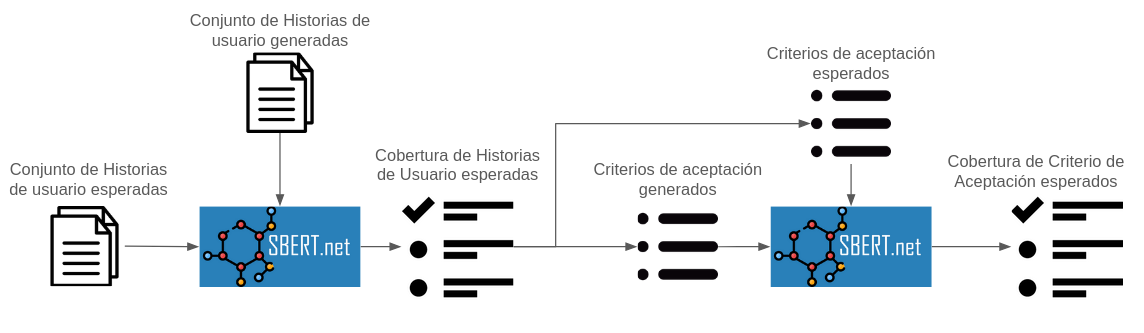
\includegraphics[
    width=\textwidth,
    height=\textheight,
    keepaspectratio
  ]{figs/sbert-hist.png}
  \caption{Diagrama de la evaluación de similitud semántica de historias y sus criterios de aceptación.}
  \label{fig:sbert-hist}
\end{figure}

Sentence-BERT también puede utilizarse para realizar búsquedas semánticas dentro de un corpus textual. En este trabajo se aprovecha esta capacidad para evaluar la cobertura de funcionalidades del sistema por parte de las historias de usuario. Para esto, se construye primero un conjunto de funcionalidades esperadas a partir del documento de requisitos (PDR). Una forma directa de obtener este conjunto es realizar una extracción manual de funcionalidades, sin embargo este proceso introduce un costo de análisis comparable al de generar manualmente las historias de usuario, lo cual reduce el beneficio de la automatización que realizamos, y de la cual estamos evaluando la calidad. Por este motivo, se adoptó un enfoque semi-automático, en el cual un modelo de lenguaje analiza el documento de requisitos y genera una lista inicial de funcionalidades del sistema. Este conjunto es posteriormente revisado y refinado por un analista humano para asegurar la correctitud y completitud del conjunto.
Una vez obtenido el conjunto de funcionalidades del dominio, se evalúa la cobertura comparando dichas funcionalidades con las historias de usuario generadas. En el diagrama \ref{fig:sbert-fun} se ilustra el proceso, que consta de los pasos:

\begin{enumerate}
    \item Un LLM analiza el documento de requisitos y genera una lista inicial de funcionalidades del sistema.
    \item Un analista humano revisa y corrige el conjunto de funcionalidades generado por el modelo.
    \item Se generan embeddings semánticos para las funcionalidades y para las historias de usuario generadas utilizando Sentence-BERT.
    \item Para cada funcionalidad se calcula la similitud semántica con todas las historias generadas, y se identifica la historia con mayor similitud semántica con la funcionalidad.
\end{enumerate}

\begin{figure}[h!]
  \centering
  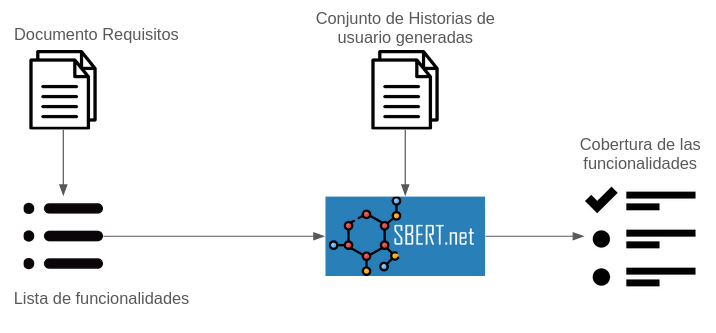
\includegraphics[
    width=\textwidth,
    height=\textheight,
    keepaspectratio
  ]{figs/sbert-fun.png}
  \caption{Diagrama de la búsqueda semántica de funcionalidades.}
  \label{fig:sbert-fun}
\end{figure}

La cobertura se determina en función del valor de similitud semántica obtenido y de una revisión manual en caso de corresponder. La evaluación se explica en la Tabla \ref{tab:similitudint}.

\begin{table}[ht]
\caption{Interpretación de cada puntaje de Similitud}
\label{tab:similitudint}
\centering
\begin{tabular}{|c|l|}
\hline
\textbf{Similitud} & \textbf{Interpretación} \\ \hline
$\geq 0.75$ & funcionalidad cubierta \\ \hline
$0.60 - 0.75$ & posible cobertura (requiere revisión manual) \\ \hline
$< 0.60$ & probablemente no cubierta (requiere revisión manual) \\ \hline
\end{tabular}
\end{table}

En los casos en que la similitud se encuentra en el rango intermedio, se realiza una revisión manual por parte de los analistas para determinar si la funcionalidad está efectivamente representada en alguna historia generada. Además, incluso en casos de baja similitud semántica se realiza una revisión manual, ya que una funcionalidad puede estar distribuida en múltiples historias de usuario o, incluso al revés, por lo que se evalúa manualmente para evitar falsos negativos.

La detección de alucinaciones o elementos incorrectos se analiza con respecto al documento de requisitos, y corresponden a elementos que no están presentes en el mismo. Para su detección se segmenta la descripción de la historia de usuario en Actor, Acción y Propósito y se marca la coherencia como Si o No para cada segmento. Se considera como una alucinación si la descripción de la historia tiene elementos que claramente no existen o son incoherentes con respecto al documento de requisitos.

Finalmente la trazabilidad será evaluada de manera manual, verificando que la referencia presente en la historia sea correcta a la sección en el documento. Marcaremos SI o NO.

\paragraph{Representación mediante grafo de similitud semántica}
Como complemento al análisis de similitud semántica utilizado para evaluar la cobertura y la alineación de las historias de usuario, se implementó una representación gráfica basada en grafos, con el objetivo de facilitar la interpretación de las relaciones entre los distintos elementos del análisis, así como también detectar fácilmente los casos problemáticos si los mismos son evidentes en el grafo, como lo puede ser por ejemplo un nodo aislado.

En el grafo modelamos tres tipos de entidades:
\begin{itemize}
    \item Funcionalidades del dominio
    \item Historias de usuario generadas
    \item Historias de usuario esperadas
\end{itemize}

Las relaciones entre los elementos se representan con aristas ponderadas, y el peso de la misma corresponde con el valor de similitud semántica calculado con Sentence-BERT.

Se definen dos tipos de relaciones:
\begin{itemize}
    \item \textbf{Cobertura:} conecta funcionalidades con historias generadas, representando en qué medida cubre una cierta funcionalidad del dominio (Nota: se mide la cobertura funcional del conjunto de historias generadas, no del conjunto esperado)
    \item \textbf{Alineación:} conecta historias generadas con historias esperadas, representando la correspondencia semántica entre ambas
\end{itemize}

Al construir el grafo se consideran solo aquellas relaciones cuya similitud supera un umbral mínimo, y para el caso de los nodos, siendo estos las entidades anteriormente definidas, se incluyen todas aunque no cuenten con aristas adyacentes. Es importante aclarar que la inclusión del grafo no introduce información adicional, sino que reorganiza los resultados obtenidos en las etapas de Alineación y Cobertura, lo que facilita la identificación visual de agrupamientos o casos borde.

\section{Procedimiento y Diagrama de evaluación}

En el diagrama \ref{fig:diag-eval} se ilustra el proceso de evaluación.
\begin{figure}[ht]
  \centering
  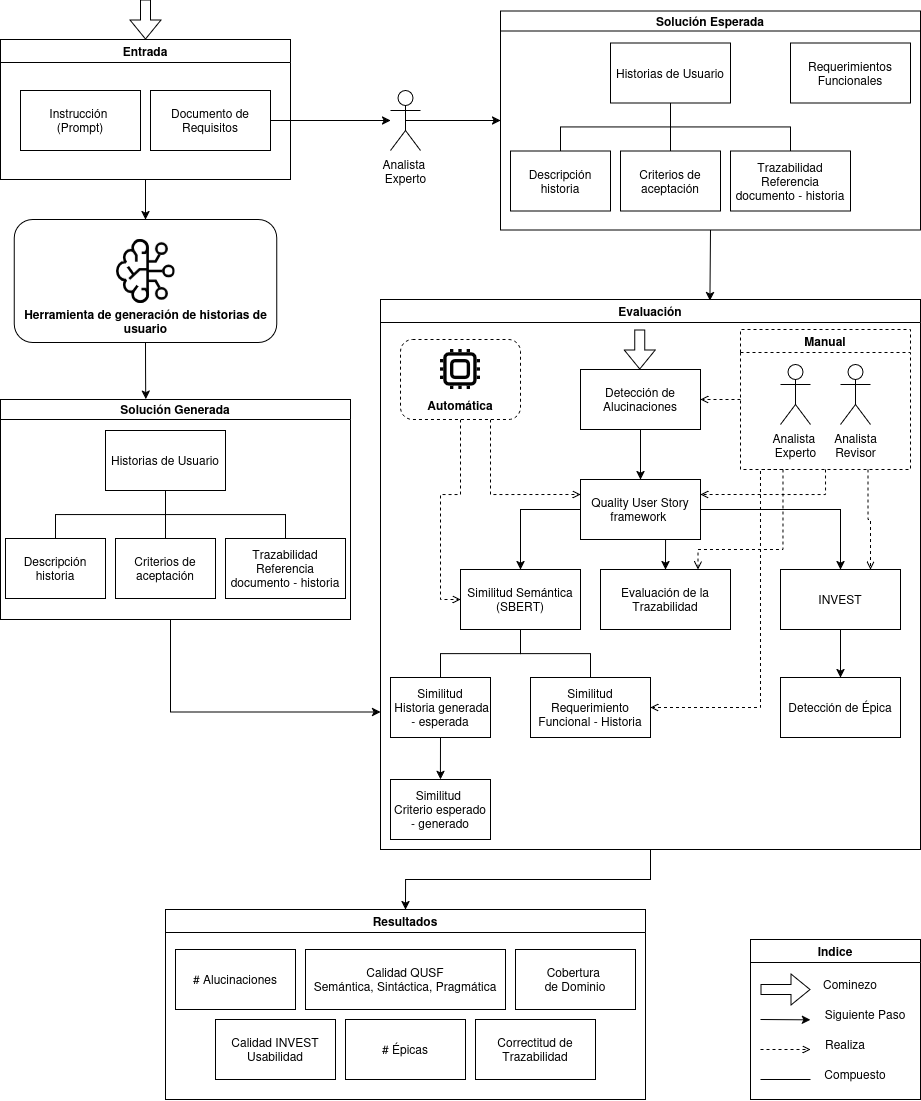
\includegraphics[
    width=\textwidth,
    height=\textheight,
    keepaspectratio
  ]{figs/Diagrama de Evaluacion.png}
  \caption{Arquitectura general del proceso de evaluación de historias de usuario.}
  \label{fig:diag-eval}
\end{figure}

La entrada se divide en dos, por un lado se tiene el documento de requisitos y por otro la instrucción o prompt, descrito en la Figura \ref{fig:prompt_simple}.
El documento de requisitos, descrito en el Capítulo~\ref{cap:herramientas} y refinado en el Capítulo~\ref{cap:central}, es utilizado por el analista experto y la herramienta de generación de historias de usuario para generar soluciones esperadas y generadas respectivamente. Por otro lado se tiene la instrucción o prompt que se utiliza para indicarle a la herramienta la salida deseada. Como se vio en la sección de selección de herramientas, no todas las herramientas requieren de un prompt pero aquellas que sí lo requieren se utiliza el prompt simple, Figura~\ref{fig:prompt_simple}.

Una vez generadas ambas soluciones, se procede a realizar la evaluación.

Como se explicó en la sección anterior, la evaluación tiene procedimientos automáticos, manuales y semi-automáticos. Para los procedimientos manuales, uno de nosotros es seleccionado como analista experto y es el encargado de evaluar la historia y otro es el analista revisor, encargado de revisar la evaluación.

El primer paso de la evaluación es la detección de alucinaciones, esto nos permite contabilizar y descartar para los pasos siguientes todas las historias consideradas como alucinaciones.

El siguiente paso es la evaluación de QUSF semántica manual del criterio Conceptually Sound (conceptualmente correcto) que nos permite identificar si la historia es coherente en sí misma. Todas aquellas que no lo cumplan serán descartadas.

Para las siguientes se evaluará QUSF, primero los criterios automáticos, utilizando la herramienta AQUSA \cite{aqusa} y luego los manuales. 

Siguiente paso será evaluar INVEST, incluyendo el criterio extra de detección de Épica para aquellas que no cumplan con el criterio Pequeño (Small).

La prueba automática de similitud semántica evalúa primero la cobertura de historia esperada y luego la cobertura de criterios dentro de esta historia.

La prueba semi-automática de búsqueda semántica de requisitos es realizada por uno de nosotros como analista a partir de la correspondencia obtenida, guardando la referencia historia-requisito y una revisión manual de los resultados obtenidos.

Finalmente la trazabilidad, de manera manual realizado por el par de analistas experto-revisor.